%%----------------------------------------------------------------------------
%% Presentatie HoGent Bedrijf en Organisatie
%%----------------------------------------------------------------------------
%% Auteur: Bert Van Vreckem [bert.vanvreckem@hogent.be]

\documentclass{beamer}

%==============================================================================
% Aanloop
%==============================================================================

%---------- Packages ----------------------------------------------------------

\usepackage{graphicx,multicol}
\usepackage{comment,enumerate,hyperref}
\usepackage{amsmath,amsfonts,amssymb}
\usepackage{tikz}
\usepackage[dutch]{babel}
\usepackage[utf8]{inputenc}
\usepackage{multirow}
\usepackage{eurosym}
\usepackage{listings}
\usepackage{lmodern}
\usepackage[T1]{fontenc}
\usepackage{textcomp}
\usepackage{framed}
\usepackage{wrapfig}
\usepackage{natbib}

%---------- Configuratie ------------------------------------------------------

\usetikzlibrary{arrows,shapes,backgrounds,positioning,shadows,calc}

\usetheme{hogent}

%---------- Commando-definities -----------------------------------------------

\newcommand{\tabitem}{~~\llap{\textbullet}~~}

%---------- Info over de presentatie ------------------------------------------

\title[Reporting]{Research Techniques\\\small Seminar session 2. Research Reporting}
\author{Anita Bernard, Jens Buysse, Bert {Van Vreckem}}
\date{AY 2016-2017}

%==============================================================================
% Inhoud presentatie
%==============================================================================

\begin{document}

%---------- Front matter ------------------------------------------------------

% Dia met het HoGent logo
\HoGentLogo

% Titeldia met faculteitslogo
\titleframe

%---------- Inhoud ------------------------------------------------------------

\begin{frame}
  \frametitle{What's on the menu today?}

  \tableofcontents
\end{frame}

\section{How to report research findings}

\subsection{Phases in writing}

\sectionframe{
\begin{center}
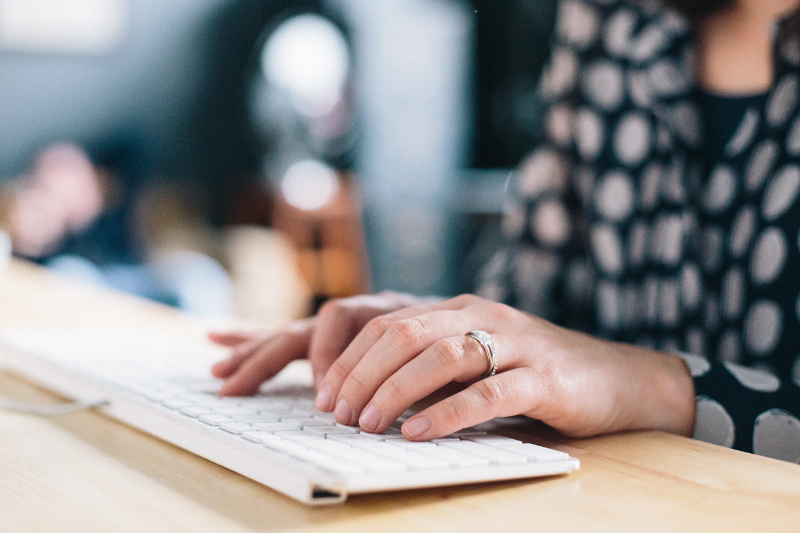
\includegraphics[width=0.8\textwidth]{img/oef2-02.jpg}
\end{center}
}

\begin{frame}
  \frametitle{Fasen in het schrijven}

  \begin{tikzpicture}[
      auto,
      thick,
      ->,
      >=stealth',
      shorten >=1pt,
      node distance=2.3cm,
    fase/.style={ shape=rectangle, fill=HoGentFBO, draw}]

    \node[fase] (1) {Planning};
    \node[fase] (2) [right of=1] {Organisation};
    \node[fase] (3) [right of=2] {Draft};
    \node[fase] (4) [right of=3] {Layout};
    \node[fase] (5) [right of=4] {Editing};

    \draw (1) -- (2);
    \draw (2) -- (3);
    \draw (3) -- (4);
    \draw (4) -- (5);
  \end{tikzpicture}
\end{frame}

\begin{frame}
  \frametitle{Planning the document}

  \begin{description}
    \item[Why?] Objective
    \item[Who?] Who's your audience? Adapt writing style and level of detail.
    \item[What?] Contents: outline or mind map
    \item[When?] Planning/work schedule
    \item[Where?] Environment
    \item[Tools?] Which tools, software? Install these!
  \end{description}
\end{frame}

\begin{frame}
  \frametitle{The audience}

  \begin{columns}[c]
    \column{.5\textwidth}

    \centering

    \textbf{The specialist}

    
\includegraphics[height=3cm]{img/oef2-04.png}

    \begin{itemize}
      \item Wants to see a lot of detail
      \item Knows technical terminology
    \end{itemize}

    \column{.5\textwidth}

    \centering

    \textbf{The non-specialist}

    
\includegraphics[height=3cm]{img/oef2-05}

    \begin{itemize}
      \item Needs more background, interpretation
      \item Needs non-technical terms
      \item Wants definitions for technical terms
    \end{itemize}
  \end{columns}
\end{frame}

\begin{frame}
  \frametitle{The audience: tips}

  Technical terminology vs. jargon

  \begin{itemize}
    \item Technical terminology: specific to the field, can be explained
    \item Jargon: wanting to impress, laziness.
  \end{itemize}

  \vfill

  \centering

  \textcolor{HoGentAccent2}{$\times$ The PS3 has 6 $\times$ SPE @3.2GHz}

  vs.

  \textcolor{HoGentAccent3}{$\checkmark$ The Playstation 3 has 6 \emph{Synergistic Processing Elements} with a clock speed of 3.2 GHz.}
\end{frame}

\begin{frame}
  \frametitle{The audience: tips}

  \begin{itemize}
    \item Explain abbreviations
    \item Add a list of abberviations (and be complete)
  \end{itemize}

  \vfill \centering

  \textbf{IP =}

  Internet Protocol?

  Intellectual Property?

  Interpersonal?

  In Progress?

  etc.

  (\url{http://www.acronymfinder.com/IP.html})

\end{frame}

\begin{frame}
  \frametitle{The audience: tips}

  Add conclusions explicitly in a separate section

  \begin{itemize}
    \item Is usually read first
    \item Even if your audience can drow conclusions themselves:
      \begin{itemize}
        \item Doesn't mean they will
        \item Other interpretations are possible
        \item Show that you are the specialist
      \end{itemize}
  \end{itemize}
\end{frame}

\subsection{Document structure}
\sectionframe{\begin{center}
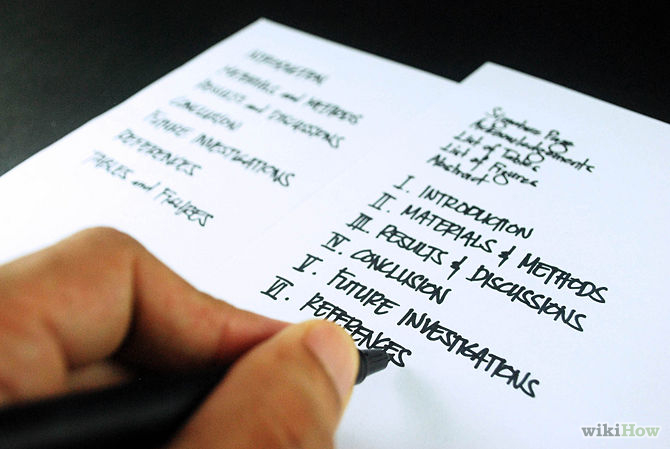
\includegraphics[width=0.8\textwidth]{img/oef2-07.jpg}
\end{center}}

\begin{frame}
  \frametitle{Organisation: document structure}

  \begin{columns}
    \column{.5\textwidth}
    \begin{center}
      Traditional approach:

      \begin{tikzpicture}[auto,thick,->,>=stealth',
          shorten >=1pt, node distance=2.3cm,
        fase/.style={shape=rectangle,inner sep=8pt,fill=HoGentAccent2,draw}]

        \node[fase] (1) {Methodology};
        \node[fase] (2) [below of=1] {Resultats};
        \node[fase] (3) [below of=2] {Conclusions};

        \draw (1) -- (2);
        \draw (2) -- (3);

      \end{tikzpicture}
    \end{center}
    \column{.5\textwidth}
    \begin{center}
      Selective approach:

      \begin{tikzpicture}[auto,thick,->,>=stealth',
          shorten >=1pt, node distance=2.3cm,
        fase/.style={shape=rectangle,inner sep=8pt,fill=HoGentAccent3,draw}]

        \node[fase] (1) {Conclusions};
        \node[fase] (2) [below of=1] {Resultats};
        \node[fase] (3) [below of=2] {Methodology};

        \draw (1) -- (2);
        \draw (2) -- (3);

      \end{tikzpicture}
    \end{center}
  \end{columns}
\end{frame}

\begin{frame}
  \frametitle{Organisation: workflow $\ne$ text order}

  Readers are interested in motivation and conclusions, usually not in the details of your approach.

  \vfill

  \begin{columns}
    \column{.25\textwidth}
    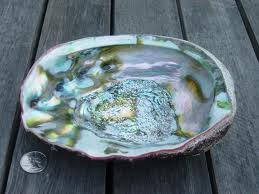
\includegraphics[width=\textwidth]{img/oef2-06}

    \column{.75\textwidth}
    \begin{quotation}
      Inspired by an abalone shell, Angela Belcher programs viruses to make elegant nanoscale structures that humans can use. Selecting for high-performing genes through directed evolution, she’s produced viruses that can construct powerful new batteries, clean hydrogen fuels and record-breaking solar cells.
    \end{quotation}
  \end{columns}
\end{frame}

\begin{frame}
  \frametitle{Organisation: document structure}

  \textbf{Short document:}

  \vfill

  \begin{columns}
    \column{.5\textwidth}
    \centering
    \begin{tikzpicture}[auto,thick,
      deel/.style={shape=rectangle,fill=HoGentAccent3,
          minimum width={width("Corpus/body")+24pt},draw}
        ]

      \node[deel] (1) [minimum height=24pt] {Introduction};
      \node[deel] (2) [below=6pt of 1,minimum height=56pt,fill=HoGentAccent1] {Body};
      \node[deel] (3) [below=6pt of 2,minimum height=24pt] {Conclusions};

    \end{tikzpicture}

    \column{.5\textwidth}
    \centering
    \begin{tikzpicture}[auto,thick,
        deel/.style={ shape=rectangle,fill=HoGentAccent3,
          minimum width={width("Corpus/body")+24pt},draw}]

      \node[deel] (1) [minimum height=24pt] {Preface};
      \node[deel] (2) [below=6pt of 1,minimum height=24pt] {Abstract};
      \node[deel] (3) [below=6pt of 2,minimum height=56pt,fill=HoGentAccent1] {Body};
      \node[deel] (4) [below=6pt of 3,minimum height=24pt] {Conclusions};

    \end{tikzpicture}

  \end{columns}
\end{frame}

\begin{frame}
  \frametitle{Organisation: document structure}

  \textbf{Long document:}

  \vfill

  \begin{columns}
    \column{.5\textwidth}
    \centering
    \begin{tikzpicture}[auto,thick,
        deel/.style={ shape=rectangle,fill=HoGentAccent3,
          minimum width={width("Corpus/body")+24pt},draw}]

      \node[deel] (1) [minimum height=24pt] {Abstract};
      \node[deel] (2) [below=6pt of 1,minimum height=24pt] {Introduction};
      \node[deel] (3) [below=6pt of 2,minimum height=56pt,fill=HoGentAccent1] {Body};
      \node[deel] (4) [below=6pt of 3,minimum height=24pt] {Conclusions};
    \end{tikzpicture}

    \column{.5\textwidth}
    \centering
    \begin{tikzpicture}[auto,thick,
        deel/.style={ shape=rectangle,fill=HoGentAccent3,
          minimum width={width("Corpus/body")+24pt},draw}]

      \node[deel] (1) [minimum height=24pt] {Preface};
      \node[deel] (2) [below=6pt of 1,minimum height=24pt] {Abstract};
      \node[deel] (3) [below=6pt of 2,minimum height=24pt] {Introduction};
      \node[deel] (4) [below=6pt of 3,minimum height=56pt,fill=HoGentAccent1] {Body};
      \node[deel] (5) [below=6pt of 4,minimum height=24pt] {Conclusions};
    \end{tikzpicture}

  \end{columns}
\end{frame}

\begin{frame}
  \frametitle{Organisation: document structure}

  Preface

  \begin{description}
    \item[Context] Why is this work important?
    \item[Need] Why did this have to be researched?
    \item[Task] What did you do exactly?
    \item[Object] What are the contents of this document?
  \end{description}

  Abstract

  \begin{description}
    \item[Result] What were the results?
    \item[Conclusion] How are these relevant for the audience?
    \item[Perspective] Are there possibilities for future work?
  \end{description}

  (short text: 1 paragraph, long text: max.~1 page)
\end{frame}

\begin{frame}
  \frametitle{Voorbeeld voorwoord/samenvatting (abstract)}

  \begin{center}
    \only<1>{Context+need}
    \only<2>{Task}
    \only<3>{Object}
    \only<4>{Conclusion}
  \end{center}

  \scriptsize
  \textbf{Energy-Efficient Resource Provisioning Algorithms for Optical Clouds}

  \alert<1>{Rising energy costs and climate change have led to an increased concern for energy-efficiency (EE). As Information and Communication Technology (ICT) is responsible for about 4\% of total energy consumption worldwide, it is essential to devise policies aimed at reducing it.} \alert<2>{In this paper, we propose a routing and scheduling algorithm for a cloud architecture, which targets minimal total energy consumption by enabling switching off unused network and/or Information Technology (IT) resources, exploiting the cloud-specific anycast principle.} \alert<3>{A detailed energy model for the entire cloud infrastructure comprising wide area optical network and IT resources is provided. This model is used to make a single-step decision on which IT end points to use for a given request, including the routing of the network connection towards these end points. Our simulations quantitatively assess the EE algorithm’s potential energy savings, but also assess the influence this may have on traditional Quality of Service parameters such as service blocking. Furthermore, we compare the one-step scheduling with traditional scheduling and routing schemes, which calculate the resource provisioning in a two-step approach (selecting first the destination IT end point, and subsequently using unicast routing towards it).} \alert<4>{We show that depending on the offered infrastructure load, our proposed one step calculation considerably lowers the total energy consumption (reduction up to 50\%) compared to the traditional iterative scheduling and routing, especially in low to medium load scenarios, without any significant increase in the service blocking.}

\end{frame}



\section{Citing sources from literature}

\subsection{Literature review: motivation}

\sectionframe{\begin{center}
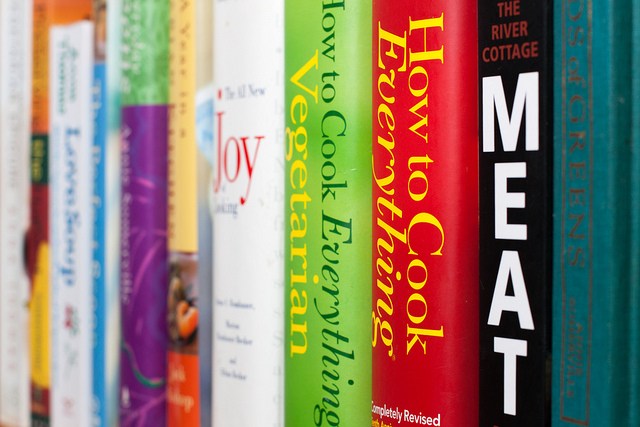
\includegraphics[width=0.8\textwidth]{img/oef2-01.png}
\end{center}}

\begin{frame}
  \frametitle{Common mistakes}

  \begin{itemize}
    \item No/incomplete bibliography
    \item Only a list of URLs
    \item Too little information to retrieve sources
    \item Unacceptable sources
    \item Bad layout
    \item No citations in the text
    \item Bibliography subdivided by publication type
    \item \ldots
  \end{itemize}
\end{frame}

\begin{frame}
  \frametitle{Objective of the literature review}

  \begin{itemize}
    \item Introduction to the subject
    \item What is the state of the art?
    \item What is the opinion of experts in the field?
    \item Clarify the subject, give context
    \item There is a problem that asks for a solution
  \end{itemize}

  \vfill

  \brightbox{\textcolor{HoGentAccent6}{Every assertion} in a literature review must be supported by citations to authoritative sources in literature.}
\end{frame}

\begin{frame}
  \frametitle{Objective of the bibliography}

  Allow readers to:

  \begin{itemize}
    \item Find the cited sources
    \item Evaluate the value of the sources independently
  \end{itemize}

  \pause

  Strict, rigid layout:

  \begin{itemize}
    \item Specific rules/styles, depending on publication (bv. IEEE, APA, Chicago Manual of Style, \ldots)
    \item Fixed order (occurrence in the text or alphabetically)
    \item A list of URLs is insufficient!
  \end{itemize}

  \pause

  \brightbox{Use \textcolor{HoGentAccent6}{reference software} to edit the bibliography!}
\end{frame}

\begin{frame}
  \frametitle{When to cite literature?}

  \begin{itemize}
    \item Definitions, first occurrence of technical terminology
    \item Verbatim quote from a source, translation/paraphrasing
      \begin{itemize}
        \item No citation $\Rightarrow$ \alert{plagiarism!}
      \end{itemize}
    \item Referring to results of previous research
    \item Every assertion about the research domain!
  \end{itemize}

  \vfill

  \brightbox{Citations give \textcolor{HoGentAccent6}{credibility} to your literature review}
\end{frame}

\subsection{Looking up and cataloguing sources}
\sectionframe{\begin{center}
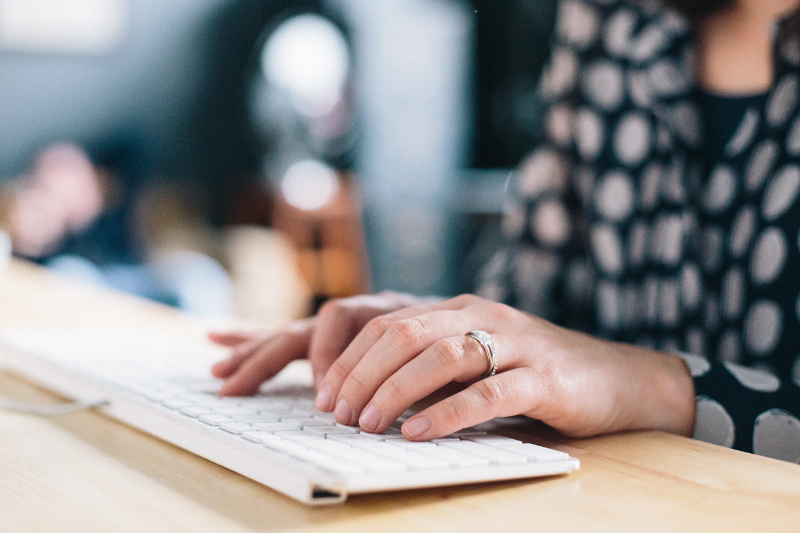
\includegraphics[width=0.8\textwidth]{img/oef2-02}
\end{center}}


\begin{frame}
  \frametitle{Types of sources}

  \begin{description}
    \item[Primary] Knowledge you've created/accumulated during your research
      \begin{itemize}
        \item experiments, surveys, interviews, \ldots
      \end{itemize}
    \item[Secundary] Publication of knowledge, research, \ldots by others
      \begin{itemize}
        \item \emph{journal} paper, article in technical publications, conference presentation, book, \ldots
      \end{itemize}
    \item[Tertiary] Indexes
      \begin{itemize}
        \item search engine, encyclopedia, library database, \ldots
      \end{itemize}
  \end{description}

  \brightbox{You're only allowed to cite \textcolor{HoGentAccent6}{secundary sources}}
\end{frame}

\begin{frame}
  \frametitle{Software}

  JabRef (\url{https://jabref.sf.net/})

  \begin{itemize}
    \item Windows, MacOS, Linux (Java)
    \item Free, open source
    \item Integrates with Bib{\TeX}, export to RTF
  \end{itemize}

  \pause

  Mendeley (\url{https://mendeley.com/})

  \begin{itemize}
    \item Windows, MacOS, Linux
    \item Freemium model
    \item Desktop + web (500MB storage space)
    \item Integration with {\LaTeX}, MS Office, Libre/OpenOffice
  \end{itemize}

  \pause

  Endnote (via \url{https://apollo.hogent.be/})
\end{frame}

\begin{frame}
  \frametitle{Looking up information}

  Start with \alert{tertiary} sources:

  \begin{itemize}
    \item Google Scholar: \url{https://scholar.google.com/}
    \item ScienceDirect: \url{https://www.sciencedirect.com/}
    \item Springer Online Journals: \url{https://link.springer.com/}
    \item Wikipedia (duh\dots)
  \end{itemize}

  \brightbox{Remark that tertiary sources, specifically Wikipedia are \textcolor{HoGentAccent6}{not} allowed as sources!}

  \pause

  \begin{itemize}
    \item No guarantee of correctness
    \item Assertions not always supported: [citation needed]
    \item Suitable as starting poing (see references at the end of the article)
  \end{itemize}
\end{frame}

\begin{frame}
  \frametitle{Tips}

  \begin{itemize}
    \item<+-> Visit HoGent library website (Dutch): \url{http://bib.hogent.be/hoekanik/}
      \begin{itemize}
        \item Search engine (\url{http://bib.hogent.be/zoeken/})
        \item Course information literacy (\url{https://bib.hogent.be/how-to/})
      \end{itemize}
    \item<+-> Apollo (\url{https://apollo.hogent.be/})
      \begin{itemize}
        \item Start apps/search engines from HoGent campus
        \item e.g.~SPSS, Endnote, Visio, Office
        \item Online journals, ebooks for which HoGent has a subscription (e.g.~ScienceDirect, SpringerLink)
      \end{itemize}
    \item<+-> Google Scholar
      \begin{itemize}
        \item Use from campus network or Apollo
        \item Check download links on the right: [PDF] or [fulltext@Hogent]
        \item Get citations in Bib{\TeX}-format (settings)
        \item Use search tools (e.g.~specify time range)
      \end{itemize}
  \end{itemize}
\end{frame}

\begin{frame}
  \frametitle{Tips (continued)}

  \begin{itemize}
    \item Presentations technical conferences (Youtube, Vimeo, Slideshare, \dots)
      \begin{itemize}
        \item vb. Google IO, WWDC, \dots
        \item Search on Lanyrd (\url{http://lanyrd.com/topics/})
      \end{itemize}
    \item<+-> Technical portal sites for it-related subjects
      \begin{itemize}
        \item e.g.~dzone.com, infoq.com, TechNet, enz.
      \end{itemize}
    \item<+-> Who are the most reputable people in the community?
      \begin{itemize}
        \item Keynotes on conferences, authors of authoritative books, enz.
        \item Follow them on Twitter
        \item Look for their blog
      \end{itemize}
    \item<+-> Technical company blogs
      \begin{itemize}
        \item Google Developers Blog, Twitter Engineering/Developer Blog, Netflix Tech Blog, \dots
      \end{itemize}
  \end{itemize}
\end{frame}


\begin{frame}
  \frametitle{Usable sources}

  (For a bachelor thesis in IT)

  \begin{description}
    \item[Journal article]<+-> academic journal, peer reviewed
    \item[Conference proceedings]<+-> paper presented on peer reviewed scientific conference
    \item[Thesis]<+-> PhD, Master, Bachelor
    \item[Manual]<+-> e.g.~of software used or discussed in your research
    \item[Book]<+-> remark: anyone can publish a book! Check the author, publisher, intended audience (Springer vs. ``for dummies'')
    \item[Presentation]<+-> by recognised professional experts, e.g.~on a technical conference (via Youtube, Vimeo, enz.)
    \item[Blog post]<+-> when written by a recognised expert
    \item[Technical magazine]<+-> remark: written by journalist, not a professional expert!
  \end{description}
\end{frame}

\begin{frame}
  \frametitle{Unusable sources}

  \begin{itemize}
    \item Any text without known author or publication year
    \item Wikipedia article
    \item Blog post from a non-expert
    \item ``White papers'' (usually not objective)
    \item Homepage of a company or product
      \begin{itemize}
        \item Belongs in the text or preferrably a footnote
      \end{itemize}
    \item \dots
  \end{itemize}
\end{frame}

\begin{frame}
  \frametitle{Checklist quality of sources}

  Do the CRAP test!

  \begin{description}
    \item[Currency] How recent is the information? Is this still state-of-the-art?
    \item[Reliability] Is the content factual or opinion? Are references to sources provided?
    \item[Relevance] Is it relevant for your research question?
    \item[Authority] Who is the author? Their credentials? Reputation?
    \item[Purpose/Point of View] What is the publisher's interest? Do they want to sell something? Fact or opinion?
  \end{description}

  Source: \url{http://loex2008collaborate.pbworks.com/w/page/18686701/The\%20CRAP\%20Test}
\end{frame}

\begin{frame}[fragile]
  \frametitle{Citations and bibliographies in {\LaTeX}}
  
  Bib{\LaTeX} and Biber

  \vspace{18pt}

  \verb|paper.tex|: Main text\\
  \verb|paper.bib|: Bibliografic database (edit with e.g.~JabRef)

  \vspace{18pt}
  
  Preamble:
  
  \begin{verbatim}
    \usepackage[backend=biber,style=apa]{biblatex}
    \DeclareLanguageMapping{english}{english-apa}
    \addbibresource{paper.bib}
  \end{verbatim}

\end{frame}

\begin{frame}[fragile]
  \frametitle{Citations and bibliographies in {\LaTeX}}
  
  \begin{itemize}
  \item Citations:
  
  \begin{itemize}
    \item \verb|\textcite{Knuth1998}| $\Rightarrow$ Knuth (1998)
    \item \verb|\autocite{Knuth1998}| $\Rightarrow$ (Knuth, 1998)
  \end{itemize}
  
  \item Add bibliography: \verb|\printbibliography|
  
  \item Compile:
  
  \begin{enumerate}
    \item `pdflatex paper` (of `latexmk -pdf`)
    \item `biber paper` selects cited sources and prepares for inclusion
    \item `pdflatex paper` to actually insert citations and bibliography
  \end{enumerate}
  \end{itemize}
  
  See the provided templates for examples!
\end{frame}

\begin{frame}
  \frametitle{Exercise}

  \begin{itemize}
    \item Look up some papers on the subject of the research project (database performance) and your bachelor thesis research proposal.
    \item Add to Bib{\TeX} file with JabRef
      \begin{itemize}
        \item Keep as much information about a source as possible: abstract, keywords, PDF, URL, \dots
      \end{itemize}
    \item Use the template for the research paper/bachelor thesis proposal in {\LaTeX}, refer in the text to sources from literature.
  \end{itemize}
\end{frame}

\end{document}
